\documentclass[11pt]{article}
\usepackage[utf8]{inputenc}
\usepackage[T1]{fontenc}
\usepackage{lmodern}
\usepackage[a4paper,margin=2.5cm]{geometry}
\usepackage{setspace}
\usepackage{graphicx}
\usepackage{array}
\usepackage{tabularx}
\usepackage{booktabs}
\usepackage{xcolor}
\usepackage{lineno}
\usepackage[hidelinks]{hyperref}
\usepackage{xurl}
\DeclareUnicodeCharacter{2212}{\ensuremath{-}}
\newcommand{\todo}[1]{\textcolor{red}{#1}}
\newcolumntype{L}[1]{>{\raggedright\arraybackslash}p{#1}}
\renewcommand{\tabularxcolumn}[1]{>{\raggedright\arraybackslash}p{#1}}
\setlength{\tabcolsep}{4pt}
\onehalfspacing
\linenumbers

\title{Reported reproducibility practices and agentic reproduction outcomes in medical and life-science papers at major ML conferences: a systematic meta-research study}
\author{Ekaterina Kondrateva\textsuperscript{1,2}, Florian Kofler\textsuperscript{1,3,4,5}, Attila Simkó\textsuperscript{6}}
\date{}
\begin{document}
\maketitle
\begin{flushleft}\small
\textsuperscript{1} Hertie AI Institute for Brain Health, University of Tübingen, Tübingen, Germany \\ \textsuperscript{2} Maastricht University, Maastricht, the Netherlands \\ \textsuperscript{3} University of Zurich, Zurich, Switzerland \\ \textsuperscript{4} Technical University of Munich, Munich, Germany \\ \textsuperscript{5} Helmholtz Munich, Munich, Germany \\ \textsuperscript{6} Umeå University, Umeå, Sweden \\ Corresponding author: Ekaterina Kondrateva, ekaterina.kondrateva@maastrichtuniversity.nl. ORCID 0000-0003-3623-6106.
\end{flushleft}
\section*{Abstract}
\textbf{Background.} Restricted data and unavailable code are common concerns in medical machine learning (ML). We examined how medical papers report reproducibility practices and what happens when independent teams attempt to reproduce them using AI agents.

\textbf{Methods.} We identified 2,170 clinical or life-science papers (together, medical papers) across nine venue-years of CVPR, ICCV, ECCV, ICLR, ICML and NeurIPS (2025 to 2026) and randomly sampled 2,170 other papers. Under a protocol frozen before sample selection, language-model coders assessed excerpts from the 3,787 retrieved full texts (87\% of the frame) for twelve reported practices, with duplicate coding of a random 25\% and of all fields below the agreement threshold. Differences were pooled across venue-years as Mantel-Haenszel risk differences with bootstrap intervals. Reproduction outcomes came from the public verdicts of the ICML 2026 agent reproduction challenge.

\textbf{Results.} Among papers with a known value, 59\% of medical papers reported releasing code, compared with 47\% of other papers (pooled difference +12 percentage points, 95\% CI +9 to +15); medical papers also more often reported variance (+25, +22 to +28) and open main data (+13, +9 to +18). Few papers in either group linked their main claims to a specific result (2.5\% versus 5.8\%). With full texts added after the first retrieval, one exploratory difference changed sign: outputs released when missing statements count as no release (from −0.2 to +0.1 percentage points, −0.8 to +1.0). In the challenge, attempted medical papers less often received a verified or falsified verdict on at least one claim (−19 percentage points, 95\% CI −28 to −10), and more of their claims were rated inconclusive (49\% versus 25\%). In exploratory analyses, adjustment for the first team's performance on other papers reduced this difference to −3.6 percentage points (−11.9 to +5.1); a difference in full verification remained and was further reduced after adjustment for coded claim requirements in a 220-paper subsample. Reported practices showed limited agreement with logbook evidence of material use (code: kappa 0.22).

\textbf{Conclusions.} Medical papers reported several reproducibility practices more often than other papers at the same venues but less often received a decided verdict in the ICML 2026 challenge. Reporting and reproduction outcomes should be assessed separately, and authors should link their main claims to the results that support them.

\section*{Introduction}
Previous studies have documented limited access to code and data in medical AI research. When a high-profile study of AI for breast cancer screening was published without its code and with few methodological details, critics argued that this undermined its scientific value~\cite{r1}. A survey of 511 papers found that ML for health compared poorly with other areas of ML on dataset and code accessibility~\cite{r2}. In the radiology journals of the RSNA, 34\% of 218 AI articles shared code and 11\% shared code that reproduced~\cite{r3}, and at the Medical Imaging with Deep Learning conference only 22\% of accepted full papers from 2018 to 2022 had a repository judged repeatable~\cite{r4}. An audit of 400 AI conference papers found that none documented all the variables a reproduction needs~\cite{r5}. NeurIPS responded with a code submission policy, a reproducibility checklist and a community-wide reproducibility challenge~\cite{r6}, and failures such as data leakage have been traced across 17 fields that apply ML~\cite{r7}.

Previous studies assessed reporting, access to research materials and, in some cases, whether shared code could be run~\cite{r3,r4}. Whether independent attempts can verify or falsify a paper's claims requires evidence from reproduction attempts. AI agents now attempt reproductions of whole papers~\cite{r8}, and agentic reproduction challenges now provide these records for large numbers of papers. In 2026 the International Conference on Machine Learning (ICML) ran an open agent reproduction challenge in which more than 1,200 participants published 6,816 reproduction logbooks on 2,226 conference papers, and an automated judge rated 35,908 claims as verified, falsified, toy (evidence at reduced scale) or inconclusive~\cite{r9}. These records provide reproduction outcomes for one venue, based on evidence submitted in logbooks and assessed by an automated judge.

We compared reported reproducibility practices between medical and other papers at the same ML venues. We then compared reproduction outcomes in the ICML 2026 challenge and explored whether differences were associated with the teams attempting the papers and the requirements of their claims. An earlier protocol of ours on the venue listings (Protocol 7, Supplementary File S1) had already found that medical papers declare a code link in the venue metadata more often than other papers (24.5\% versus 16.9\% across twelve venue-years, +7.4 percentage points, 95\% CI +5.8 to +9.0). For the practices that the metadata does not show (open data, weights and variance), we nonetheless prespecified the common assumption, that medical papers report them less often, as directional hypotheses. The full-text analysis did not support these directional hypotheses: medical papers reported the practices more often. Reproduction outcomes were less favourable for medical papers. We examined this difference in post hoc analyses, with interpretation criteria recorded before each analysis was run.

\section*{Methods}
Protocol 9 was frozen in a public repository before selection of the study sample, full-text retrieval and coding. It was developed after the results of earlier protocols on the same challenge were known. The study is reported following the PRISMA 2020 statement~\cite{r10} where its items apply to a meta-research study of published papers. The protocol, its amendments and the reporting checklist are described in Appendix A.

\subsection*{Information sources and eligibility}
The sources were the public virtual-site listings of nine venue-years: CVPR 2025, ICCV 2025, ECCV 2026, ICLR 2025, ICLR 2026, ICML 2025, ICML 2026, NeurIPS 2025 and NeurIPS 2026 (40,290 papers after removing duplicates and papers without an abstract). Abstracts missing from the 2026 listings were taken from the challenge's paper metadata (ICML 2026) or from each paper's page on the venue site (ICLR 2026, NeurIPS 2026, ECCV 2026).

A paper was a candidate for the medical group if its venue topic was a health, biology, neuroscience or chemistry topic, or its title or abstract matched a prespecified regular expression of clinical and biological terms (Supplementary File S1, Protocol 7). This gave 5,530 candidates. Each candidate was labelled \texttt{clinical}, \texttt{life\_science} or \texttt{no} from title and abstract only by a blind language-model coder; a second blind coder labelled a random 25\% of candidates (1,633 papers over the whole listing; agreement 97.7\%, Cohen's kappa 0.96~\cite{r11}; threshold 0.80) and disagreements were adjudicated with a written reason. Of the candidates, 1,013 were labelled clinical and 1,157 life science, together the 2,170 medical papers, and 3,360 were excluded. To estimate how many medical papers the prefilter missed, both coders labelled a random 200 non-candidates; none was medical (0 of 200, 95\% Wilson interval~\cite{r12} 0 to 1.9\%). The comparison group was a random sample of 2,170 non-candidates, allocated to venue-years in proportion to the medical counts (seed 20261019).

\subsection*{Full-text retrieval and excerpts}
Full texts were retrieved in a fixed order: arXiv HTML, then arXiv PDF (arXiv identifier from a title search, accepted at a normalised title similarity of at least 0.95 and an arXiv year no earlier than the venue year minus one; ambiguous matches excluded), then the open proceedings (CVF, PMLR). OpenReview was not scraped. To complete coverage, a recovery step frozen before any further request (Note 9-23) added proceedings.neurips.cc (NeurIPS 2025) and proceedings.iclr.cc (ICLR 2025 and 2026) under the same title rule, the OpenReview API PDF accessed with the first author's own account (public papers only), and a unique OpenAlex work with an open-access PDF; access refusals and bot checks counted as no full text. Papers without a retrievable full text remained in the study frame but were excluded from documentation coding. We reported retrieval failures by group and venue-year. From each full text an excerpt of at most 15,000 characters was built from the end of the introduction, sections whose heading concerned availability, reproducibility, ethics, data, setup, implementation, training, compute or limitations, the NeurIPS checklist items on reproducibility, and paragraphs on seeds and repeated runs, with a truncation flag per paper.

\subsection*{Data items and coding}
Each excerpt was coded on twelve fields (Table 1 lists the indicators): whether main claims were listed and linked to evidence; code (released, promised, no); main data access (open, credentialed or on request, private, synthetic only); an experiment on open data; release of synthetic or sample data, of weights and of outputs; variance (several seeds, error bars or intervals); environment (versions or container); compute (amount, hardware only, none); compute tier; and training-set scale. Every field allowed \texttt{unclear}. Coders used stated text only; a named dataset without stated access terms was \texttt{unclear}.

\begin{table}[htbp]
\centering\footnotesize
\renewcommand{\thetable}{1}
\caption{Reported reproducibility practices, medical versus other papers, nine venue-years. Medical papers had higher reporting rates for nine of ten indicators. Shares among papers with a known value; pooled difference is the Mantel-Haenszel risk difference over venue-years with a 95\% paper bootstrap interval.}\label{tab:table1}
\begin{tabularx}{\textwidth}{XL{1.75cm}L{1.75cm}L{3.55cm}L{1.75cm}}
\toprule
\textbf{Practice} & \textbf{Medical, \% (n known)} & \textbf{Other, \% (n known)} & \textbf{Pooled difference, points (95\% CI)} & \textbf{Unclear, medical / other} \\ \midrule
Main claims listed and linked to evidence & 2.5 (1831) & 5.8 (1893) & −3.3 (−4.6 to −2.1) & 39 / 24 \\
Code released & 59.3 (1756) & 46.8 (1812) & +12.1 (+8.8 to +15.4) & 114 / 105 \\
Main data openly available & 82.5 (1048) & 67.9 (719) & +13.5 (+9.5 to +17.7) & 822 / 1198 \\
Experiment on open data & 90.9 (1215) & 76.6 (1031) & +13.3 (+10.1 to +16.2) & 655 / 886 \\
Synthetic or sample data released & 22.1 (199) & 11.5 (485) & +10.3 (+3.9 to +16.8) & 1671 / 1432 \\
Weights released & 50.8 (323) & 19.3 (533) & +30.7 (+24.4 to +37.1) & 1547 / 1384 \\
Outputs released & 21.3 (178) & 8.4 (450) & +14.6 (+8.2 to +21.1) & 1692 / 1467 \\
Variance reported & 68.5 (1506) & 43.6 (1529) & +24.9 (+21.7 to +28.0) & 364 / 388 \\
Environment stated & 19.0 (748) & 9.5 (950) & +9.9 (+6.7 to +13.4) & 1122 / 967 \\
Compute amount stated & 22.2 (1302) & 16.9 (1473) & +5.7 (+2.8 to +8.5) & 568 / 444 \\
\bottomrule
\end{tabularx}
\end{table}

Coding was done by language-model subagents (claude-sonnet-5-5), 20 papers per batch, with venue, year and group hidden. Coder 1 coded all papers and coder 2 a random 25\% (943 papers). Agreement exceeded the prespecified kappa threshold of 0.80 for code release (0.85), main data access (0.82) and weights (0.96). We therefore used coder 1's labels for these fields. Agreement was below the threshold for variance (0.73) and compute (0.72). These fields underwent duplicate coding across the full sample, followed by blinded adjudication of all 1,553 disagreements by a language model (claude-opus-5-5) that saw the two labels in random order and gave a reason.

\subsection*{Reproduction outcomes}
Outcomes came from the public verdict snapshot of the ICML 2026 agent reproduction challenge retrieved on 17 October 2026~\cite{r9}. In the challenge, participants chose papers from the conference list, for each of which the organisers had extracted core claims from the abstract as checkable targets, and reproduced them with AI agents, with or without human steering, on compute credits provided by the organisers~\cite{r9}. Each attempt was published as a logbook (a Trackio Space with the write-up, the code that ran, the artifacts it produced and, optionally, the agent's execution trace)~\cite{r9}. An automated judge (GLM-5.2) then read each logbook, treated the logbook's own self-assessment as untrusted, and gave each claim one of four verdicts: verified, falsified, toy (supported only by a reduced-scale or synthetic-data run) or inconclusive; the organisers re-checked every claimed falsification themselves~\cite{r9}. On fixed input this judge agreed with itself well (Krippendorff's alpha 0.874), whereas verdicts on the same claim from different logbooks agreed poorly (alpha 0.229), a difference its author attributes mainly to the evidence that different attempts produce rather than to the judge~\cite{r13}.

A paper was classified as attempted if it had at least one logbook, and as decided if at least one claim received a verified or falsified verdict. We classified it as fully verified if at least one logbook verified every claim assessed in that logbook. Logbooks were deduplicated, and the first author's own logbooks were excluded because the first author took part in the challenge. Of the 6,341 ICML 2026 papers, 622 candidates labelled \texttt{no} were excluded, leaving 328 medical and 5,391 other papers.

To assess agreement between reported practices and material use (reference standard), two blind coders read the logbooks of the 222 attempted ICML 2026 papers in the frame and coded whether the authors' code was obtained and run, the main data obtained, and weights used; disagreements were adjudicated as above. A further random 300 attempted ICML 2026 papers outside the frame were added later under a prespecified extension (Note 9-17).

\subsection*{Quantitative synthesis}
For each indicator we computed the share of papers with the practice among papers with a known value (\texttt{unclear} excluded and counted), by group and venue-year, with Wilson intervals~\cite{r12}. The difference between groups was pooled over the nine venue-years as a Mantel-Haenszel risk difference~\cite{r14}, with a 95\% interval from 2,000 paper bootstrap resamples within strata (seed 20261017; results identical under two hash seeds). Three directional hypotheses were prespecified: medical papers report open main data, release weights and report variance less often; each was to be supported only if the pooled interval excluded zero in that direction.

For reproduction outcomes the primary analysis compared the decided share of attempted papers by group, unadjusted and adjusted for compute tier and data scale. Post hoc analyses (Notes 9-9 to 9-15) examined how many teams attempted each paper, the first team's performance on other papers, within-team claim-level differences, and the requirements of each claim. We measured first-team performance as the proportion of its other attempted papers with a decided claim in that team's latest logbook, excluding the focal paper. For claim requirements, two blind coders classified every distinct claim text of the 110 attempted medical papers and of 110 randomly drawn attempted other papers as needing inference only, retraining, large-scale runs, or analysis only; the claim texts reveal the subject, so these coders were blind to the group label but not to the domain. We prespecified a descriptive criterion for interpreting adjusted estimates: the absolute difference had to decrease by more than half, and its 95\% interval had to include zero. Meeting this criterion was not interpreted as evidence of causation. Adversarial checks (Notes 9-12 and 9-14) stated in advance what would refute each main claim. After an internal review of this manuscript, three further post hoc analyses were frozen before their intervals were computed (Note 9-22): documentation differences among papers reporting a training-set size, which we used as an operational definition of empirical papers; release fields with \texttt{unclear} treated as no reported release; and the mix of verdicts by group. We did not correct for multiple comparisons; the post hoc analyses are exploratory.

Two further post hoc analyses, requested after the main results were known, were frozen with their codebooks before any paper was coded (Notes 9-24 and 9-26). First, two blind coders assigned one application topic from a fixed list of 13 to each of the 2,170 medical papers on its title and abstract. Second, they coded all 4,340 papers on three axes: the primary type of input data (14 labels), the primary methodological family (13 labels, including causal inference and trials and biostatistical inference) and every model architecture the paper builds or adapts (11 labels, several allowed). Papers whose architecture was not named in the abstract were coded again on their excerpt. Coders were blind to venue, year and group, and every disagreement was adjudicated blind by a third model. We compared label shares between groups (Mantel-Haenszel over venue-years) and tested venue by topic with adjusted standardised residuals, reading a cell as over- or under-represented only at an absolute residual of at least 3. To ask whether the reporting differences reflect the data and methods each group uses, we repeated the pooled differences for code, open main data, weights and variance with strata of venue-year by data type and venue-year by method. These analyses are descriptive and exploratory.

\subsection*{Ethics}
The study used published papers and public challenge records, and involved no human participants and no patient data. The challenge records include the public account names under which participants published their logbooks. We used them only to group logbooks by team; no account name is reported in this paper or in the paper-level table. No ethics review was sought for this secondary analysis of public records.

\section*{Results}
Figure 1 summarises the main results.

\begin{figure}[htbp]
\centering
\setcounter{figure}{0}
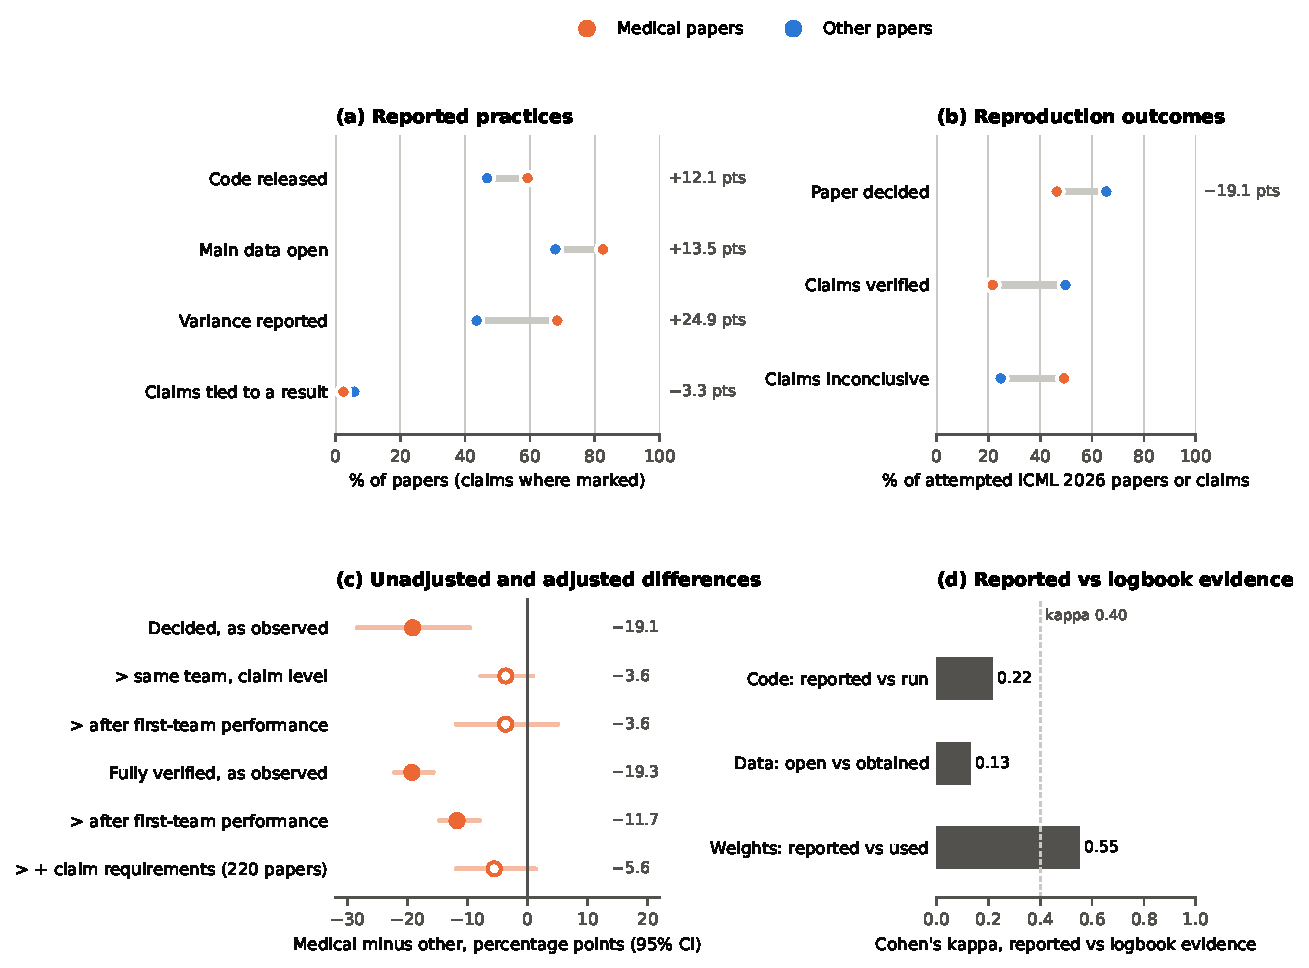
\includegraphics[width=\textwidth]{figures/fig1.pdf}
\caption{Reported reproducibility practices and reproduction outcomes in medical and other papers. (a) Among papers with a known value, medical papers (orange) more often reported code release, open main data and variance than other papers (blue); both groups rarely linked their claims to a specific result. (b) In the ICML 2026 challenge, attempted medical papers less often had a decided claim, with fewer claims verified and more rated inconclusive. (c) Within-team comparisons and adjustment for first-team performance reduced the estimated difference in decided outcomes. In the 220-paper subsample, additional adjustment for claim requirements further reduced the full-verification difference. Filled circles: interval excludes zero; open circles: interval includes zero. (d) Agreement between reported practices and logbook evidence of material use; the dashed line marks kappa 0.40.}\label{fig:1}
\end{figure}

\subsection*{Study selection}
Figure 2 shows the flow of papers. Of the 4,340 papers in the frame, full texts were retrieved for 3,787 (1,870 medical and 1,917 other papers): 3,278 in the first retrieval and 509 in the recovery step (Note 9-25). Of the remaining 553, 130 had no match on any source and 423 could not be checked on OpenAlex because its daily request quota was reached, after every other source had returned nothing. Retrieval was complete or nearly complete for every venue-year except NeurIPS 2026 (177 of 431 medical and 221 of 431 other papers), whose papers were not public before the conference, and ECCV 2026 (85 of 129 and 97 of 129) (Table A1). It was lower for medical than for other papers (86.2\% against 88.3\%). Of the excerpts, 3,261 reached the 15,000-character limit.

\begin{figure}[htbp]
\centering
\setcounter{figure}{1}
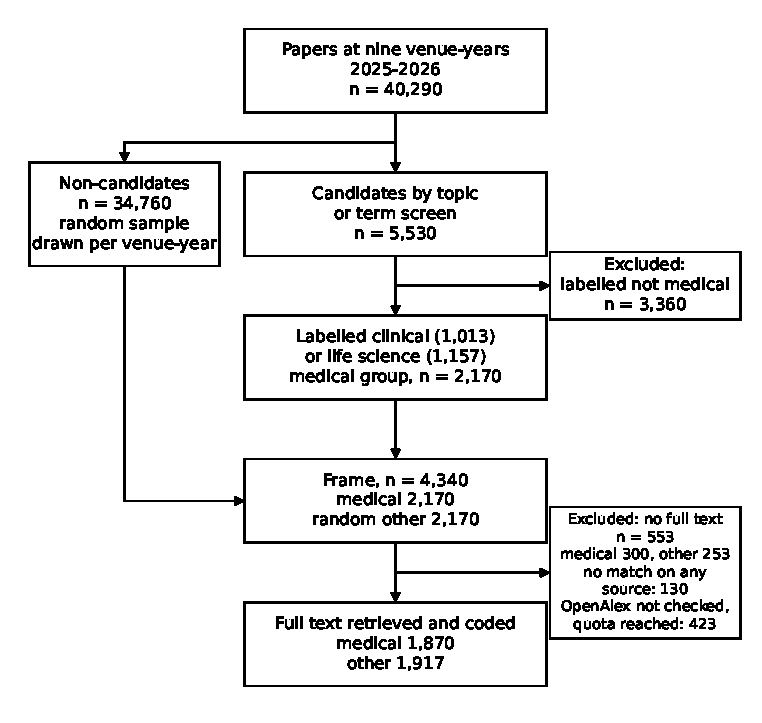
\includegraphics[width=\textwidth]{figures/fig2.pdf}
\caption{Study selection and full-text retrieval. Full texts were retrieved for 3,787 of 4,340 papers, 509 of them in the recovery step (Note 9-23). Retrieval was lower for medical papers than for other papers (86.2\% versus 88.3\%).}\label{fig:2}
\end{figure}

\subsection*{Reported practices}
Table 1 and Figure 3 give every indicator. Among papers with a known value for each field, medical papers more often reported code release (59.3\% versus 46.8\%; pooled difference +12.1 percentage points, 95\% CI +8.8 to +15.4), open main data (82.5\% versus 67.9\%; +13.5, +9.5 to +17.7), weights release (50.8\% versus 19.3\%; +30.7, +24.4 to +37.1) and variance (68.5\% versus 43.6\%; +24.9, +21.7 to +28.0). Medical papers had higher reporting rates for nine of the ten indicators. None of the three prespecified directional hypotheses was supported. For each practice, the estimated difference favoured medical papers. The exception was claims listed and each linked to a table, figure or theorem, which was rare in both groups (2.5\% versus 5.8\%; −3.3, −4.6 to −2.1). Compute was rarely reported by either group (22.2\% and 16.9\% gave an amount), and most papers did not report their compute tier (1,611 of 1,870 medical papers).

\begin{figure}[htbp]
\centering
\setcounter{figure}{2}
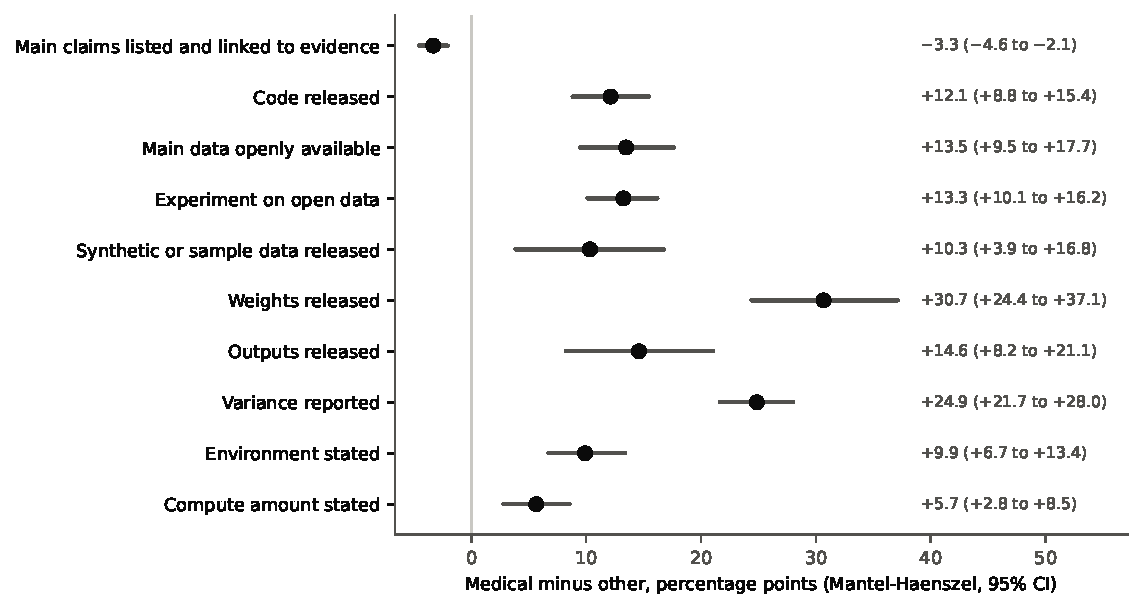
\includegraphics[width=\textwidth]{figures/fig3.pdf}
\caption{Differences in reported practices among papers with a known value for each indicator. Medical papers had higher reporting rates for nine of ten indicators and a lower rate of explicit links between claims and supporting results. Mantel-Haenszel risk difference, medical minus other, over nine venue-years with 95\% bootstrap intervals. Filled circles: interval excludes zero.}\label{fig:3}
\end{figure}

The four differences remained positive across the specified sensitivity analyses (Note 9-12, F1): leaving out each venue-year in turn, using coder 1's or coder 2's codes alone, restricting to papers whose excerpt was not truncated, and stratifying by venue-year and excerpt length. They also remained positive for clinical and life-science papers separately and for vision venues (CVPR, ICCV, ECCV) and learning venues (ICLR, ICML, NeurIPS) separately, except open main data at vision venues (+7.5, −1.8 to +18.1).

A training-set size was not reported in 44.7\% of other papers and 28.8\% of medical papers. Among the 1,331 medical and 1,060 other papers reporting a training-set size, all four differences remained positive: code +10.2 percentage points (+6.2 to +14.2), open main data +5.5 (+0.7 to +10.1), weights +23.9 (+15.5 to +32.1) and variance +24.9 (+20.7 to +29.2) (Table 4). Release fields were often not reported at all: a statement on weights could be coded for 323 of 1,870 medical papers. In a sensitivity analysis treating \texttt{unclear} as no reported release, medical papers still more often reported open main data (46.3\% versus 25.5\%; +20.7, +17.7 to +23.7). The estimated weights difference decreased to +3.3 percentage points (+1.7 to +4.9). Intervals for sample or synthetic data (−0.6, −1.6 to +0.5) and outputs (+0.1, −0.8 to +1.0) included zero; the outputs estimate was −0.2 in the first retrieval.

\begin{table}[htbp]
\centering\footnotesize
\renewcommand{\thetable}{4}
\caption{Sensitivity analyses of reported practices, medical minus other, Mantel-Haenszel over venue-years, percentage points with 95\% CI (post hoc, Note 9-22): main analysis, papers reporting a training-set size, and all coded papers with unclear treated as no reported release.}\label{tab:table4}
\begin{tabularx}{\textwidth}{XL{3.55cm}L{3.55cm}L{3.9cm}}
\toprule
\textbf{Practice} & \textbf{Main analysis: known value} & \textbf{Papers reporting a training-set size} & \textbf{All coded papers, unclear as no reported release} \\ \midrule
Code released & +12.1 (+8.8 to +15.4) & +10.2 (+6.2 to +14.2) &  \\
Main data openly available & +13.5 (+9.5 to +17.7) & +5.5 (+0.7 to +10.1) & 46.3 vs 25.5\%; +20.7 (+17.7 to +23.7) \\
Weights released & +30.7 (+24.4 to +37.1) & +23.9 (+15.5 to +32.1) & 8.8 vs 5.4\%; +3.3 (+1.7 to +4.9) \\
Variance reported & +24.9 (+21.7 to +28.0) & +24.9 (+20.7 to +29.2) &  \\
Synthetic or sample data released & +10.3 (+3.9 to +16.8) &  & 2.4 vs 2.9\%; −0.6 (−1.6 to +0.5) \\
Outputs released & +14.6 (+8.2 to +21.1) &  & 2.0 vs 2.0\%; +0.1 (−0.8 to +1.0) \\
\bottomrule
\end{tabularx}
\end{table}

\subsection*{Reproduction outcomes in the ICML 2026 challenge}
Medical papers were attempted about as often as other papers (110 of 328, 33.5\%, against 1,821 of 5,391, 33.8\%) but by fewer teams (mean 1.5 against 3.3 teams per attempted paper). Among attempted papers, 46.4\% of medical papers were decided against 65.5\% of other papers, a difference of −19.1 percentage points (95\% CI −28.4 to −9.6; permutation p < 0.001). The estimated difference was −23.6 percentage points for clinical papers (95\% CI −36.2 to −10.9) and −13.4 for life-science papers (−27.5 to +0.9), and it was −19.1 (−29.7 to −8.7) when every logbook of the team with the most medical attempts was dropped. The difference was also negative for full verification (−19.3, −22.1 to −15.7) and for any falsified claim (−10.8, −16.9 to −4.1). Claims of medical papers were rated verified in 21.7\% against 49.7\% and inconclusive in 49.2\% against 24.8\%. Toy verdicts accounted for 25.5\% of medical claims and 20.9\% of other claims (difference +4.7 percentage points, 95\% CI −0.6 to +10.7). In the prespecified analysis on the 222 attempted frame papers, the difference was −17.0 percentage points (−29.7 to −4.4); adjustment for reported compute tier and data scale changed it to −14.7 (−28.8 to −0.5).

Table 2 and Figure 4 show the post hoc analyses. In comparisons within the same team, the difference in the proportion of claims decided decreased from −29.1 to −3.6 percentage points (95\% CI −7.8 to +0.8). The first team to take up a medical paper had a decided claim on 40.0\% of its other attempted papers, against 60.3\% for teams first on other papers (−20.3, −26.0 to −14.3). Among 903 papers attempted by at least two teams, the team with better performance on other papers was more likely to obtain a decided verdict on the same paper (difference +32.3 percentage points, 95\% CI +29.9 to +34.7). After adjustment for the first team's performance on other papers, the difference in papers with a decided claim decreased from −19.1 to −3.6 percentage points (95\% CI −11.9 to +5.1). A difference in full verification remained (−11.7, −14.7 to −8.0). Adjustment for whether a paper listed and linked its claims changed the decided difference to −15.3 percentage points (−28.5 to −2.2; 216 frame papers); few attempted papers in either group linked each claim to a result (3 medical and 9 other papers).

\begin{table}[htbp]
\centering\footnotesize
\renewcommand{\thetable}{2}
\caption{Unadjusted and adjusted differences in reproduction outcomes of attempted ICML 2026 papers, medical minus other (post hoc analyses, Notes 9-9 to 9-15). Rows marked subsample use the 220 papers with coded claim requirements.}\label{tab:table2}
\begin{tabularx}{\textwidth}{XL{3.6cm}}
\toprule
\textbf{Outcome and adjustment} & \textbf{Medical minus other, points (95\% CI)} \\ \midrule
Decided, all attempted papers (110 vs 1,821), unadjusted & −19.1 (−28.4 to −9.6) \\
Decided, clinical papers only & −23.6 (−36.2 to −10.9) \\
Decided, life-science papers only & −13.4 (−27.5 to +0.9) \\
Decided, adjusted for number of teams & −9.2 (−18.1 to +0.4) \\
Decided, adjusted for first-team performance & −3.6 (−11.9 to +5.1) \\
Fully verified, all attempted papers, unadjusted & −19.3 (−22.1 to −15.7) \\
Fully verified, all attempted papers, adjusted for first-team performance & −11.7 (−14.7 to −8.0) \\
Fully verified, claim-coded subsample (220 papers), unadjusted & −19.1 (−27.3 to −10.9) \\
Fully verified, subsample, adjusted for first-team performance & −13.0 (−20.7 to −5.1) \\
Fully verified, subsample, adjusted for first-team performance and claim requirements & −5.6 (−11.9 to +1.4) \\
Claim decided, unadjusted (claim level) & −29.1 (−37.9 to −20.2) \\
Claim decided, within team (claim level) & −3.6 (−7.8 to +0.8) \\
\bottomrule
\end{tabularx}
\end{table}

\begin{figure}[htbp]
\centering
\setcounter{figure}{3}
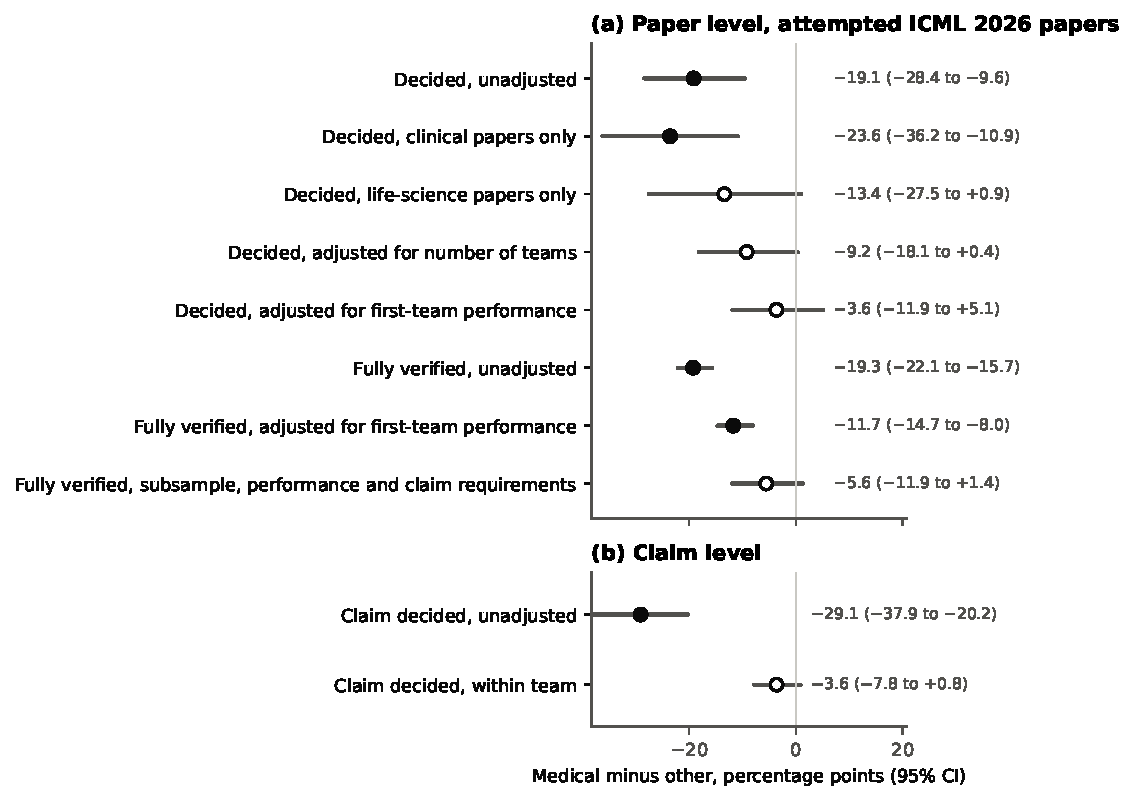
\includegraphics[width=\textwidth]{figures/fig4.pdf}
\caption{Unadjusted and adjusted differences in reproduction outcomes between medical and other papers. Estimates are shown at paper level for decided and fully verified outcomes, and at claim level before and after comparisons within teams. Estimates use all attempted ICML 2026 papers (or their clinical or life-science subset, where labelled), except the last paper-level row, which uses the 220-paper subsample with coded claim requirements. Filled circles: interval excludes zero.}\label{fig:4}
\end{figure}

In the 220-paper subsample, coders classified 56.7\% of medical claims and 39.1\% of other claims as requiring retraining or large-scale runs (difference +17.6 percentage points, 95\% CI +9.7 to +25.8), and 19.3\% and 45.3\% as checkable by analysis alone. In this subsample, the full-verification difference was −19.1 percentage points, −13.0 (−20.7 to −5.1) after adjustment for first-team performance, and −5.6 (−11.9 to +1.4) after adjustment for both first-team performance and claim requirements.

\subsection*{Reported practices against logbook evidence}
On the 222 attempted frame papers, agreement between reported code release and logbook evidence that the authors' code had been run was limited (kappa 0.22; n = 162; sensitivity 0.74, specificity 0.56). Agreement between reported open data and logbook evidence that the data were obtained was also limited (kappa 0.13, n = 89), and higher for weights (kappa 0.55, n = 43). Pooled with the 300 extension papers, the kappas were 0.28 (n = 347), 0.16 (n = 163) and 0.60 (n = 118). In the NeurIPS subset, agreement between checklist answers on code availability and the coded release statements was also limited (kappa 0.21, n = 153) (Table 3).

\begin{table}[htbp]
\centering\footnotesize
\renewcommand{\thetable}{3}
\caption{Agreement between reported practices and logbook evidence of material use, 222 attempted ICML 2026 frame papers; the last column pools them with the 300-paper extension sample. Agreement was limited for code and data and higher for weights.}\label{tab:table3}
\begin{tabularx}{\textwidth}{XL{0.7cm}L{1.6cm}L{1.6cm}L{1.0cm}L{2.4cm}}
\toprule
\textbf{Stated in full text vs obtained by reproducers} & \textbf{n} & \textbf{Sensitivity} & \textbf{Specificity} & \textbf{Kappa} & \textbf{Kappa pooled with extension (n)} \\ \midrule
Code released vs authors' code run & 162 & 0.74 & 0.56 & 0.22 & 0.28 (347) \\
Main data open vs data obtained & 89 & 0.87 & 0.27 & 0.13 & 0.16 (163) \\
Weights released vs weights used & 43 & 0.75 & 0.92 & 0.55 & 0.60 (118) \\
NeurIPS checklist item 5 vs code released & 153 & 0.80 & 0.50 & 0.21 &  \\
\bottomrule
\end{tabularx}
\end{table}

\subsection*{Topics, data and methods (post hoc, exploratory)}
The topic coders agreed on 92.0\% of medical papers (kappa 0.91; 173 disagreements adjudicated). The most frequent topics were neuroscience (380 papers, 17.5\%), radiology (367, 16.9\%), proteins (250, 11.5\%) and genomics and omics (222, 10.2\%). Topics differed by venue (chi-square 662.5, 60 degrees of freedom; Figure 5). Radiology was over-represented at CVPR, ICCV and ECCV (adjusted residuals 10.5, 7.6 and 10.7) and under-represented at ICLR, ICML and NeurIPS. Proteins were over-represented at ICLR and ICML, molecules at ICLR, genomics and omics at ICML, and neuroscience at NeurIPS (4.6). Figure 6 maps the abstracts.

\begin{figure}[htbp]
\centering
\setcounter{figure}{4}
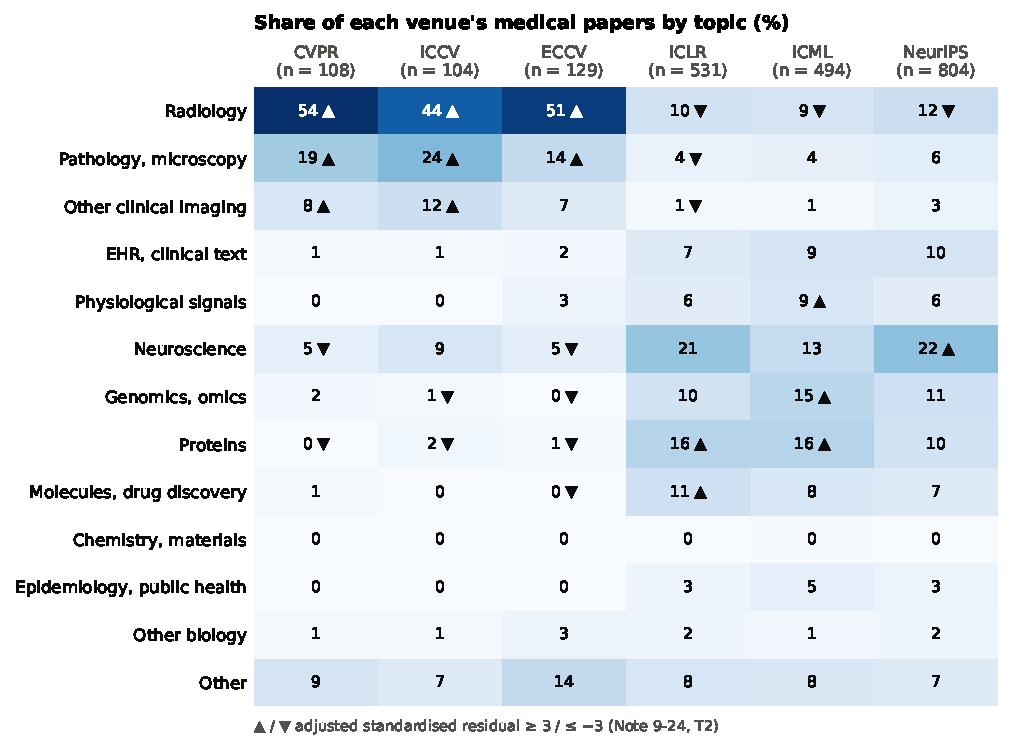
\includegraphics[width=\textwidth]{figures/fig_topics_venue.pdf}
\caption{Topics of the 2,170 medical papers by venue (years pooled), post hoc. Share of each topic per venue; triangles mark adjusted standardised residuals of at least 3 in absolute value. Topics were coded blind from title and abstract by two coders with adjudication. Radiology and pathology dominate the computer vision venues, and proteins, molecules, genomics and neuroscience the learning venues.}\label{fig:5}
\end{figure}

\begin{figure}[htbp]
\centering
\setcounter{figure}{5}
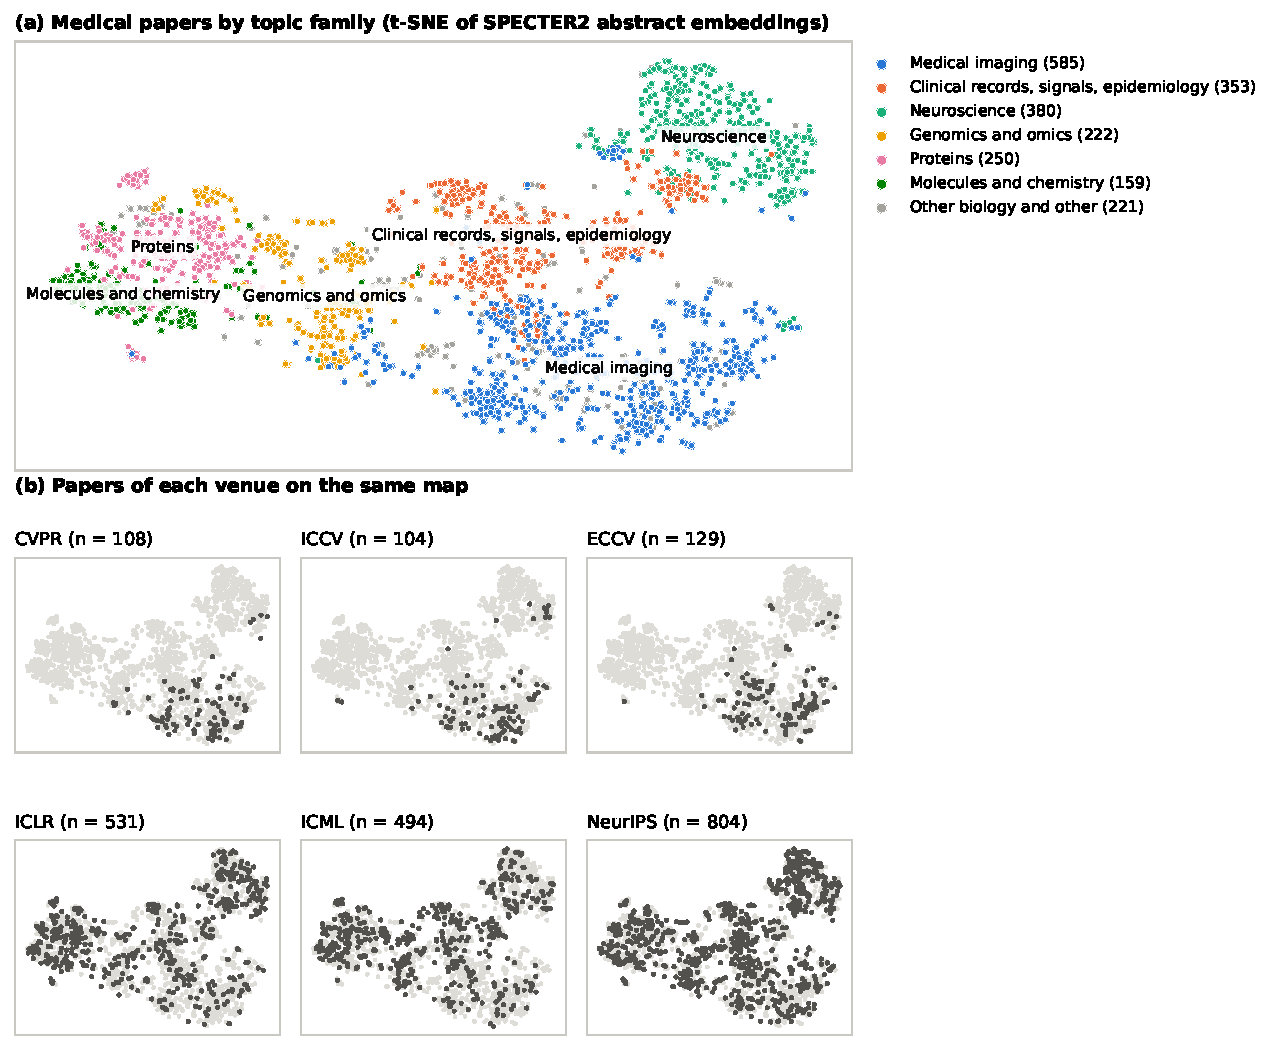
\includegraphics[width=\textwidth]{figures/fig_topics_map.pdf}
\caption{Map of the medical papers' abstracts, post hoc. t-SNE of SPECTER2 embeddings of title and abstract, coloured by topic (left) and by venue (right). The map illustrates Figure 5 and was not used for inference.}\label{fig:6}
\end{figure}

For the three axes, agreement was high for data type (kappa 0.91) and method (kappa 0.88), and lower for architecture (exact agreement on the label set 0.81); 1,630 item-axis disagreements were adjudicated. Medical papers more often used molecular graphs (+12.1 percentage points, +10.4 to +13.7), time series (+10.1, +8.5 to +11.7) and volumetric images (+8.1, +7.1 to +9.3), and less often text (−17.0, −19.0 to −15.1) or no data or synthetic data (−12.4, −14.1 to −10.8) (Figure 7). They more often reported representation learning (+12.8, +10.8 to +14.7) and less often optimisation and efficiency (−10.4, −11.9 to −9.0) or theory (−8.5, −9.9 to −7.3). Causal inference and trials (2.6\% versus 1.2\%) and biostatistical inference (2.4\% versus 1.3\%) were rare in both groups. Language or vision-language models were built or adapted in 20.5\% of medical and 36.6\% of other papers.

\begin{figure}[htbp]
\centering
\setcounter{figure}{6}
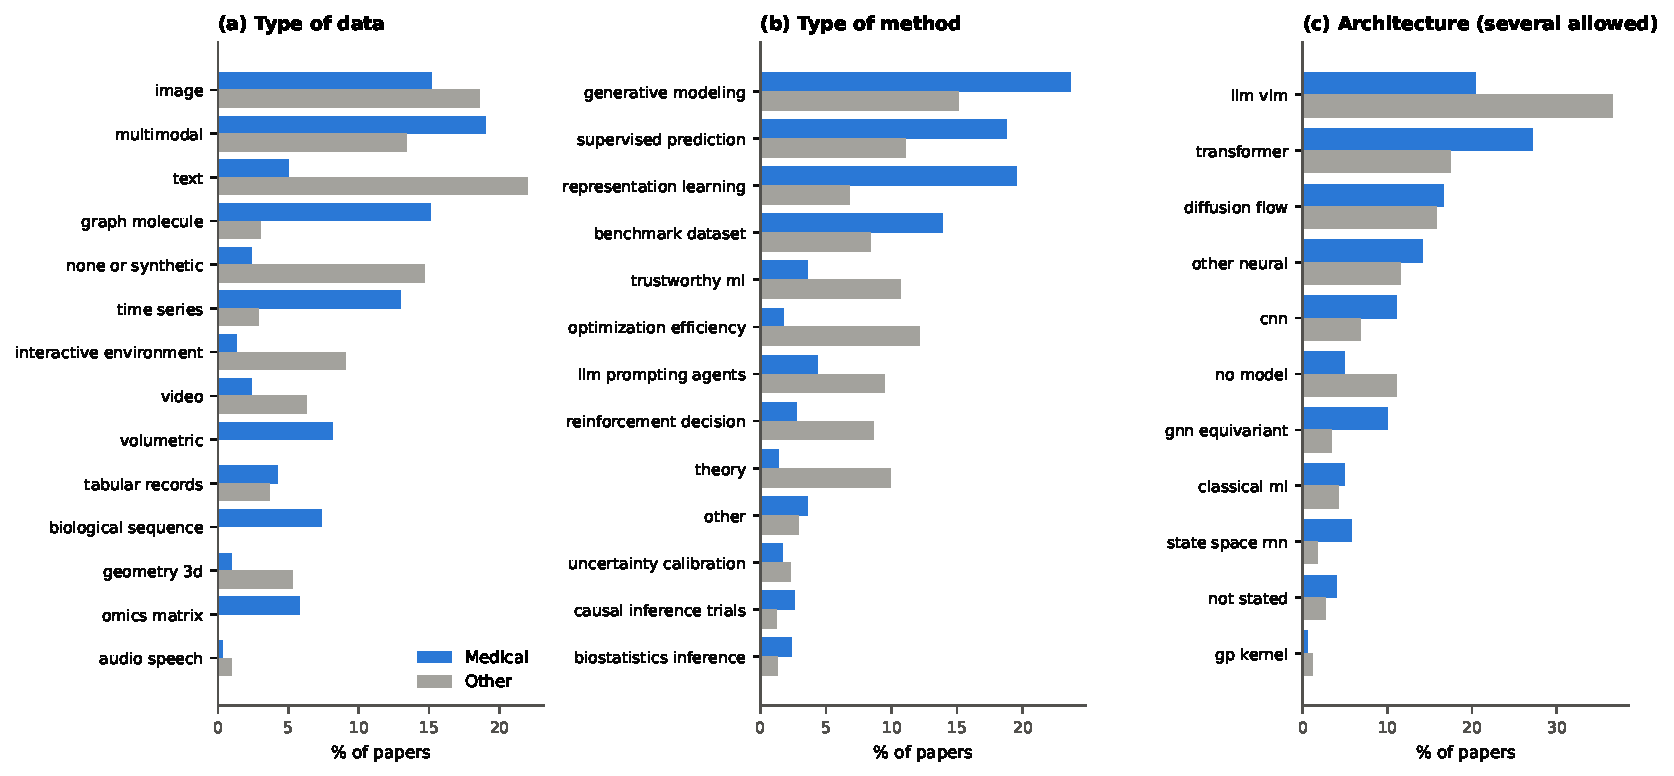
\includegraphics[width=\textwidth]{figures/fig_axes.pdf}
\caption{Type of data, method and architecture of all 4,340 papers, post hoc. Share of each label in medical and other papers. Architecture allows several labels per paper.}\label{fig:7}
\end{figure}

With strata of venue-year by method, the four reporting differences remained positive: code +11.7 percentage points (+8.2 to +15.2), open main data +4.7 (+0.9 to +8.7), weights +14.3 (+7.8 to +21.0) and variance +24.4. With strata of venue-year by data type, code (+10.8), weights (+20.3, +12.7 to +28.0) and variance (+21.2) stayed positive, but the open main data difference of +13.5 reversed to −6.1 percentage points (−10.3 to −2.0). Within the same type of data, medical papers did not report open main data more often than other papers. This analysis was not planned and its strata are small; we read it as a hypothesis about where the open-data difference comes from, not as an estimate to replace the main one.

\section*{Discussion}
\subsection*{Principal findings}
Medical papers more often reported code release, open main data and variance than other papers at the same venues. These differences remained among papers reporting a training-set size. Statements about weights and other releases were often missing, and their estimated differences were sensitive to how missing values were handled.

In the ICML 2026 challenge, medical papers were attempted by fewer teams and less often received a verified or falsified verdict on at least one claim. Adjustment for the first team's performance on other papers reduced this difference from −19.1 to −3.6 percentage points. A difference in full verification remained. In the 220-paper subsample, this difference was further reduced after adjustment for the coded computational requirements of claims. These exploratory results identify factors associated with reproduction outcomes; they do not establish why the outcomes differed.

\subsection*{Comparison with earlier work}
An earlier survey found weaker sharing in ML for health than in other ML areas~\cite{r2}, and audits of medical imaging found low rates of shared and working code in radiology journals~\cite{r3} and at a medical imaging conference~\cite{r4}. Our frame differs: it covers only papers accepted at general ML venues, several of which have introduced code policies and checklists~\cite{r6}, and it compares medical papers with other papers at the same venues and in the same years. In our sample, medical papers more often reported code release, open main data and variance. Earlier audits assessed reporting~\cite{r5} or tested whether shared code ran~\cite{r3,r4}; here reported practices could be compared with logbook evidence from independent reproduction attempts, and agreement for code was limited (kappa 0.22). PaperBench evaluated agents on a fixed set of 20 ICML 2024 Spotlight and Oral papers~\cite{r8}; in an open challenge, by contrast, participants choose what to attempt. In this challenge, paper domain was associated with the performance of the teams attempting a paper and with the requirements of its claims.

\subsection*{Implications}
An unadjusted verification rate combines paper characteristics with differences in who attempts the papers and how the attempts are conducted. It should therefore be interpreted alongside team participation, performance on other papers and claim requirements. Reporting guidelines for ML-based science~\cite{r15}, for clinical prediction models that use ML~\cite{r16} and for deep learning in medical imaging~\cite{r17} concern what authors report. We propose the following reporting changes based on the gaps identified in this study. We did not test whether these changes improve reproduction outcomes.

\subsection*{Recommendations}
For authors of medical ML papers:

\begin{itemize}
\item List the main claims and link each to its supporting table, figure or theorem. This mapping was present in 2.5\% of medical papers and 5.8\% of other papers.
\item Specify how the main data can be accessed: openly, with credentials, on request or privately. Access could not be coded from the text for 822 of 1,870 medical papers.
\item State whether weights, outputs and sample or synthetic data are released, including when they are not. Weights were not reported in 1,547 of 1,870 medical papers.
\item Report the hardware and runtime required to check each main claim. The compute tier was not reported in 1,611 of 1,870 medical papers.
\end{itemize}

For organisers of reproduction challenges and for logbook formats such as Trackio:

\begin{itemize}
\item Link each extracted claim to the specific result being checked, including its table, figure or theorem. The challenge used claims extracted from abstracts~\cite{r9}.
\item Record in each logbook, per claim, whether the authors' code was run, the main data obtained and the weights used.
\item For each claim, record the type of check: inference, retraining, large-scale runs or analysis only. Report the compute used and give a reason for an inconclusive verdict.
\item Report the number of teams attempting each paper and their performance on other papers. Present unadjusted domain comparisons alongside analyses accounting for these factors.
\end{itemize}

For venues:

\begin{itemize}
\item Use explicit categories for data access and material release, and ask authors to link each main claim to its supporting result. In the NeurIPS subset, agreement between checklist answers on code availability and the coded release statements was limited (kappa 0.22).
\end{itemize}

\subsection*{Strengths and limitations}
The frame included all papers identified as clinical or life science by the screening procedure, together with a random comparison sample allocated across the same venue-years. The protocol and coding rules were fixed before sample selection, every coding decision is public, and the main reporting differences remained positive across the specified sensitivity analyses. The study has several limitations. All coders, adjudicators and the challenge judge are language models; agreement between coders was high, but they may share systematic errors, and verdicts on the same claim from different logbooks agreed poorly in the challenge as a whole~\cite{r13}. More comparison papers lacked a reported training-set size. Restricting the analysis to papers reporting one reduced the differences for code, open data and weights, while all four estimated differences remained positive. Full texts were missing for 13\% of the frame, mostly at NeurIPS 2026, whose papers were not yet public, and at ECCV 2026; retrieval was lower for medical papers. Papers recovered from proceedings and OpenReview reported variance more often than papers of the first, mostly arXiv, retrieval (exploratory, Note 9-25); the estimates on the first retrieval alone were close to the main ones. Many excerpts reached the character limit, which may have omitted relevant release statements. Release fields were often coded as \texttt{unclear}, and several estimated differences decreased when these values were treated as no reported release. Coded practices are what authors report, not working artifacts. Performance on other papers may reflect the agents, human input, compute and paper selection of a team. We did not measure these components separately. The frame covers six venues (CVPR, ICCV, ECCV, ICLR, ICML and NeurIPS); the same frame procedure and codebook can be extended to other major AI venues, such as COLT, AAAI, IJCAI, ACL, EMNLP, KDD, ICRA, HRI and ACM MM. The reproduction outcomes come from one venue, one challenge and one judge model, and the challenge's participants chose what to attempt. Protocol 9 was developed after the results of earlier protocols on the same challenge were known, including the higher rate of code links in medical papers. The higher rate of open main data in medical papers did not hold within the same type of data in an exploratory analysis, so it may reflect the data each group works with rather than reporting habits. Analyses of team performance and claim requirements were post hoc and were not adjusted for multiple comparisons. They used different samples: all attempted papers for team performance and a 220-paper subsample for claim requirements. The adjusted estimates are exploratory and do not establish causal explanations.

\subsection*{Conclusions}
Medical papers more often reported several reproducibility practices than other papers at the same ML venues. In the ICML 2026 challenge, they less often received a verified or falsified verdict on at least one claim. Exploratory analyses associated these outcomes with team performance and, in a subsample, the computational requirements of claims. Reporting practices and reproduction outcomes should therefore be assessed separately. Authors should link their main claims to specific results, and reproduction reports should document team participation, material use and the resources required for each check.

\section*{Declarations}
\textbf{Data availability.} The repository contains the paper-level table for all 4,340 papers, claim codes, frozen protocol, analysis code and aggregate results: \url{https://github.com/kondratevakate/life-science-at-ml-venues} \todo{[DOI to be added on release]}. The paper-level table includes identifiers, titles, group labels, full-text retrieval status and coded fields. Code is released under the MIT licence; data and text are released under CC BY 4.0. Abstracts and full texts were retrieved from public conference websites, arXiv, open proceedings, the OpenReview API and open-access copies listed by OpenAlex and are not redistributed for copyright reasons; the repository contains the retrieval scripts and SHA-256 manifests of the retrieved files. Challenge verdicts come from the public snapshot of the ICML 2026 agent reproduction challenge retrieved on 17 October 2026. No patient data were used.

\textbf{Code availability.} All analysis code is in the repository above; \texttt{python setup\_data.py} links the retrieved inputs and each analysis script reproduces its result file. Rerunning all Protocol 9 analyses from the committed codes gave byte-identical results.

\textbf{Ethics approval and consent.} Not applicable: secondary analysis of published papers and public challenge records, with no human participants and no patient data. Public account names of challenge participants were used only to group logbooks by team and are not reported.

\textbf{Competing interests.} EK took part in the ICML 2026 agent reproduction challenge as a reproducer; her own logbooks were excluded from all analyses. \todo{[Other competing interests of all authors to be added.]}

\textbf{Funding.} \todo{[To be added.]}

\textbf{Author contributions.} \todo{[To be added in CRediT terms.]}

\textbf{Use of AI tools.} Language models produced domain labels, documentation codes, logbook codes and claim classifications. We used claude-sonnet-5-5 for coding and claude-opus-5-5 for adjudication under the published protocol and prompts. Claude also assisted with analysis code and manuscript drafts. The authors checked every number against the result files and take responsibility for the content.

\clearpage
\begin{thebibliography}{99}
\bibitem{r1} Haibe-Kains B, Adam GA, Hosny A, Khodakarami F, Massive Analysis Quality Control (MAQC) Society Board of Directors, Waldron L, et al. Transparency and reproducibility in artificial intelligence. Nature. 2020;586(7829):E14–6. doi:10.1038/s41586-020-2766-y
\bibitem{r2} McDermott MBA, Wang S, Marinsek N, Ranganath R, Foschini L, Ghassemi M. Reproducibility in machine learning for health research: still a ways to go. Sci Transl Med. 2021;13(586):eabb1655. doi:10.1126/scitranslmed.abb1655
\bibitem{r3} Venkatesh K, Santomartino SM, Sulam J, Yi PH. Code and data sharing practices in the radiology artificial intelligence literature: a meta-research study. Radiol Artif Intell. 2022;4(5):e220081. doi:10.1148/ryai.220081
\bibitem{r4} Simkó A, Garpebring A, Jonsson J, Nyholm T, Löfstedt T. Reproducibility of the methods in medical imaging with deep learning. In: Medical Imaging with Deep Learning. Proceedings of Machine Learning Research. 2024;227:95–106.
\bibitem{r5} Gundersen OE, Kjensmo S. State of the art: reproducibility in artificial intelligence. Proc AAAI Conf Artif Intell. 2018;32(1). doi:10.1609/aaai.v32i1.11503
\bibitem{r6} Pineau J, Vincent-Lamarre P, Sinha K, Larivière V, Beygelzimer A, d'Alché-Buc F, et al. Improving reproducibility in machine learning research (a report from the NeurIPS 2019 reproducibility program). J Mach Learn Res. 2021;22(164):1–20.
\bibitem{r7} Kapoor S, Narayanan A. Leakage and the reproducibility crisis in machine-learning-based science. Patterns. 2023;4(9):100804. doi:10.1016/j.patter.2023.100804
\bibitem{r8} Starace G, Jaffe O, Sherburn D, Aung J, Chan JS, Maksin L, et al. PaperBench: evaluating AI's ability to replicate AI research. In: Proceedings of the 42nd International Conference on Machine Learning. PMLR; 2025. p. 56843–73.
\bibitem{r9} Abid A. What we learned by reproducing 2,200 papers from ICML [Internet]. Hugging Face; 2026 Aug 13. Available from: \url{https://huggingface.co/blog/icml-2026-open-reproductions}
\bibitem{r10} Page MJ, McKenzie JE, Bossuyt PM, Boutron I, Hoffmann TC, Mulrow CD, et al. The PRISMA 2020 statement: an updated guideline for reporting systematic reviews. BMJ. 2021;372:n71. doi:10.1136/bmj.n71
\bibitem{r11} Cohen J. A coefficient of agreement for nominal scales. Educ Psychol Meas. 1960;20(1):37–46. doi:10.1177/001316446002000104
\bibitem{r12} Wilson EB. Probable inference, the law of succession, and statistical inference. J Am Stat Assoc. 1927;22(158):209–12. doi:10.1080/01621459.1927.10502953
\bibitem{r13} Umoh EH. Who verifies the verifier? Measuring LLM-as-judge reliability across 32,688 automated research verdicts \todo{[poster]}. AWS-MLU Fall AI Teaching and Research Symposium; 2026 Sep 22; Arlington, VA. Available from: \url{https://github.com/SturdivantAI/who-verifies-the-verifier}
\bibitem{r14} Mantel N, Haenszel W. Statistical aspects of the analysis of data from retrospective studies of disease. J Natl Cancer Inst. 1959;22(4):719–48. doi:10.1093/jnci/22.4.719
\bibitem{r15} Kapoor S, Cantrell EM, Peng K, Pham TH, Bail CA, Gundersen OE, et al. REFORMS: consensus-based recommendations for machine-learning-based science. Sci Adv. 2024;10(18):eadk3452. doi:10.1126/sciadv.adk3452
\bibitem{r16} Collins GS, Moons KGM, Dhiman P, Riley RD, Beam AL, Van Calster B, et al. TRIPOD+AI statement: updated guidance for reporting clinical prediction models that use regression or machine learning methods. BMJ. 2024;385:e078378. doi:10.1136/bmj-2023-078378
\bibitem{r17} Moassefi M, Singh Y, Conte GM, Khosravi B, Rouzrokh P, Vahdati S, et al. Checklist for reproducibility of deep learning in medical imaging. J Imaging Inform Med. 2024;37(4):1664–73. doi:10.1007/s10278-024-01065-2
\end{thebibliography}
\section*{Appendix A. Protocol and reporting}
Protocol 9 was frozen on 19 October 2026, before sample selection, full-text retrieval and coding (commit 839281e in kondratevakate/icml-2026-repro). It was developed after the results of Protocols 6 to 8 on the same challenge were known. Subsequent decisions were recorded in dated protocol notes (Notes 9-1 to 9-27) before the corresponding analyses were run. Analyses added after the original protocol are labelled post hoc and exploratory. The study was not registered in a review register. We report it following the PRISMA 2020 statement~\cite{r10} where its items apply to a meta-research study of published papers; the completed checklist is Supplementary File S2. The protocol, all notes and their commit history are in Supplementary File S1 and the repository. Table A1 gives the papers in the frame and with a coded full text per venue-year.

\begin{table}[htbp]
\centering\footnotesize
\renewcommand{\thetable}{A1}
\caption{Papers in the frame and with a coded full text, by group and venue-year. Retrieval was nearly complete where open proceedings exist and lowest at NeurIPS 2026.}\label{tab:tablea1}
\begin{tabularx}{\textwidth}{XL{4.2cm}L{4.2cm}}
\toprule
\textbf{Venue-year} & \textbf{Medical: frame / full text} & \textbf{Other: frame / full text} \\ \midrule
cvpr-2025 & 108 / 108 & 108 / 108 \\
iccv-2025 & 104 / 104 & 104 / 104 \\
eccv-2026 & 129 / 85 & 129 / 97 \\
iclr-2025 & 222 / 221 & 222 / 219 \\
iclr-2026 & 309 / 308 & 309 / 305 \\
icml-2025 & 166 / 166 & 166 / 165 \\
icml-2026 & 328 / 328 & 328 / 328 \\
neurips-2025 & 373 / 373 & 373 / 370 \\
neurips-2026 & 431 / 177 & 431 / 221 \\
Total & 2170 / 1870 & 2170 / 1917 \\
\bottomrule
\end{tabularx}
\end{table}

\end{document}